\section{Further model results}\label{app:model}

These figures give the full results behind the tables and text of the model sections. All come from the same planar model or geometry model with assumed parameters (Table~\ref{tab:4}); they compare wheel configurations and are not real-world thresholds. ``With fork'' is the main model of the Voiager 5; ``no fork'' is the rigid version kept for comparison.

\subsection{Geometry model}

\begin{figure}[htbp]
\centering
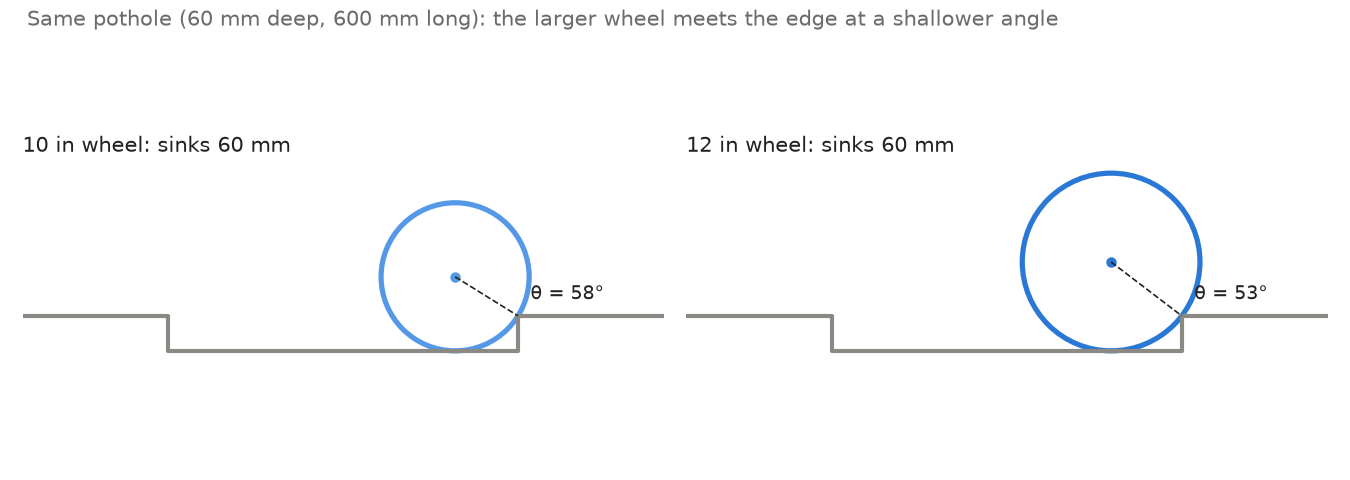
\includegraphics[width=\linewidth]{sim/geom_schematic.png}
\caption{Geometry model schematic: a 10 in and a 12 in rigid wheel at the far edge of the same 60 mm deep, 600 mm long pothole, drawn sunk to full depth for illustration. The larger wheel meets the edge at a shallower angle $\theta$.}\label{fig:E1}
\end{figure}

\begin{figure}[htbp]
\centering
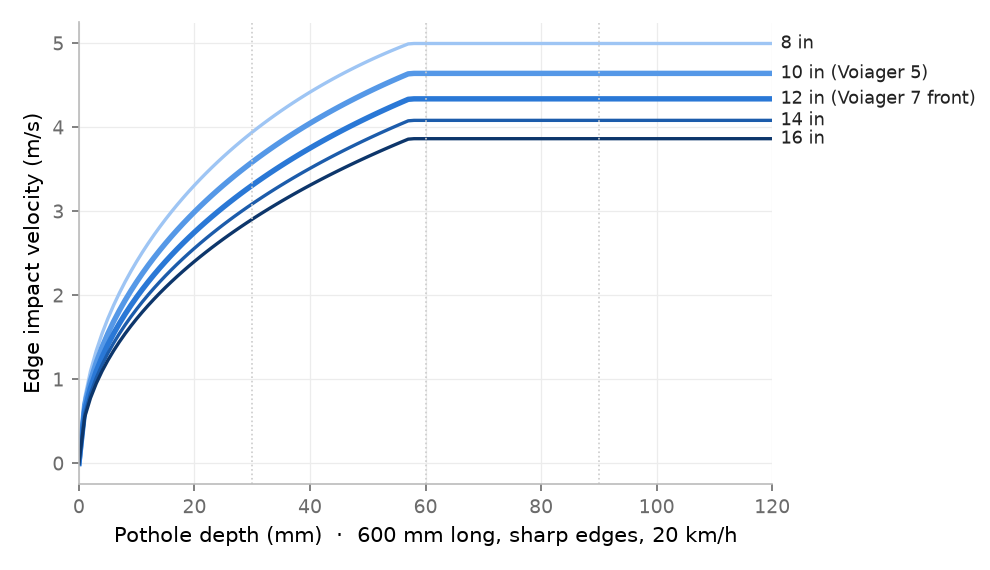
\includegraphics[width=\linewidth]{sim/geom_impact_velocity.png}
\caption{Geometry model: front-wheel edge impact velocity against pothole depth by wheel diameter (600 mm long, 20 km/h).}\label{fig:E2}
\end{figure}

\begin{figure}[htbp]
\centering
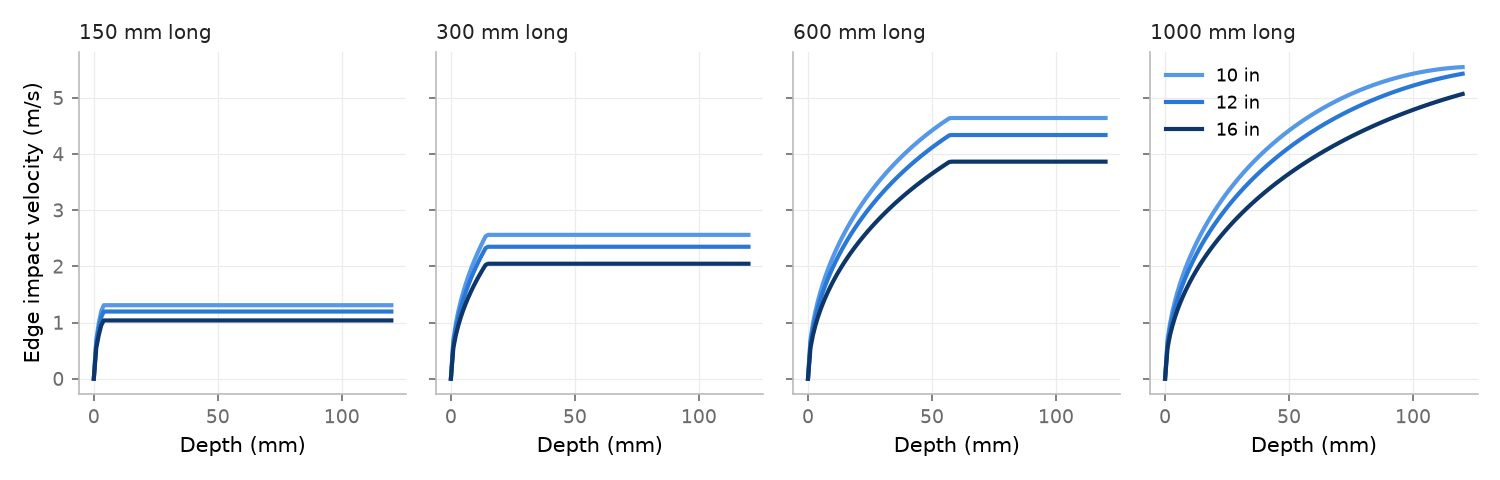
\includegraphics[width=\linewidth]{sim/geom_by_length.png}
\caption{Geometry model: edge impact velocity by pothole depth and length, 20 km/h. Short potholes limit how far the wheel can drop at speed.}\label{fig:E3}
\end{figure}

\FloatBarrier
\subsection{Main sweep}

\begin{figure}[htbp]
\centering
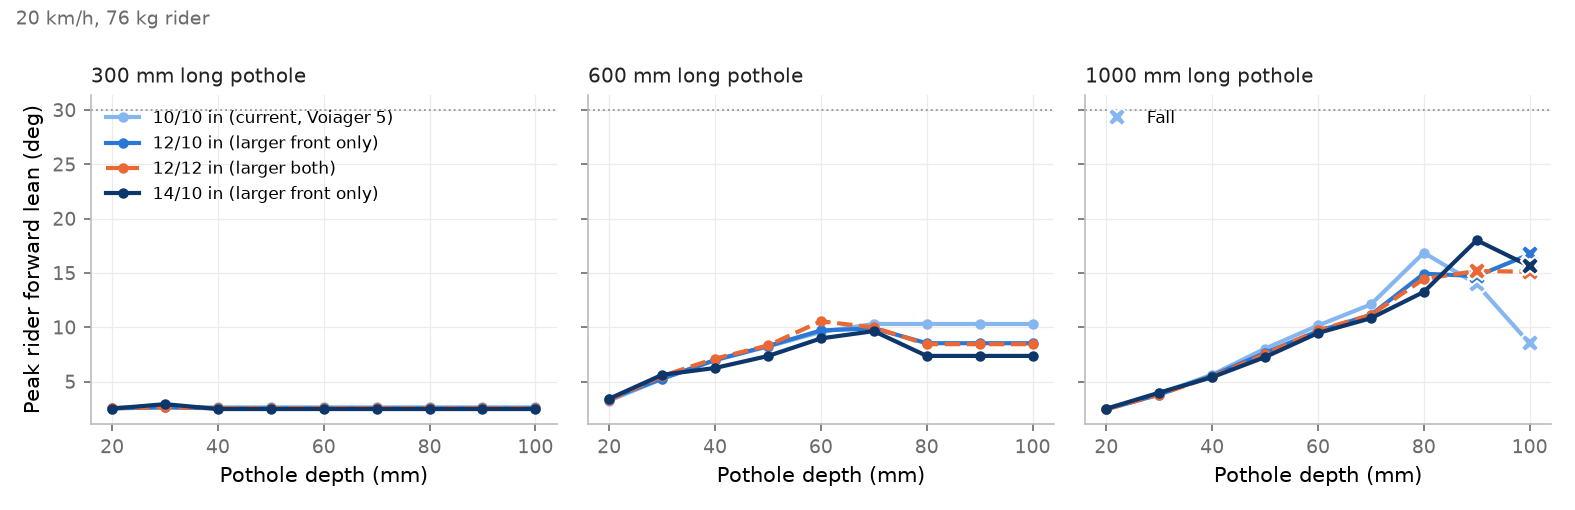
\includegraphics[width=\linewidth]{sim/sweep_lean_fork.png}
\caption{Main sweep, with front suspension (main model): peak forward lean of the rider by pothole depth and length at 20 km/h; X marks a fall. Planar model with assumed parameters (Table~\ref{tab:4}); relative comparison of wheel configurations only, not real-world thresholds.}\label{fig:Eleanfork}
\end{figure}

\begin{figure}[htbp]
\centering
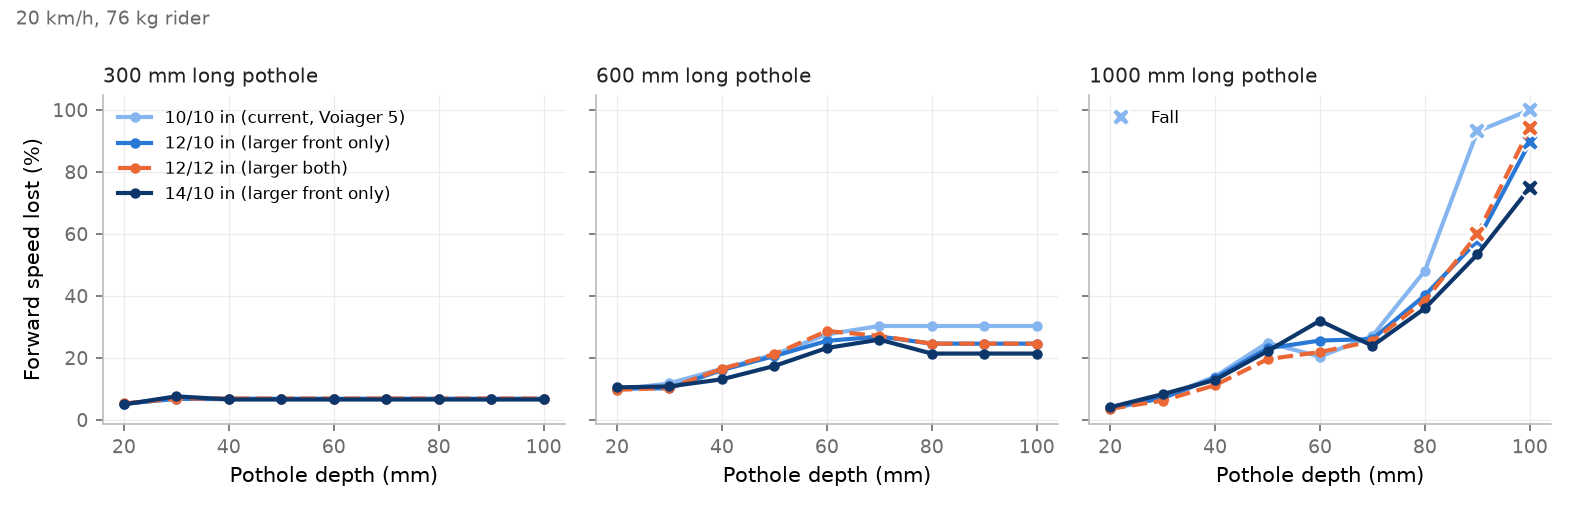
\includegraphics[width=\linewidth]{sim/sweep_speedloss_fork.png}
\caption{Main sweep, with front suspension (main model): forward speed lost crossing the pothole. Planar model with assumed parameters (Table~\ref{tab:4}); relative comparison of wheel configurations only, not real-world thresholds.}\label{fig:Espeedfork}
\end{figure}

\begin{figure}[htbp]
\centering
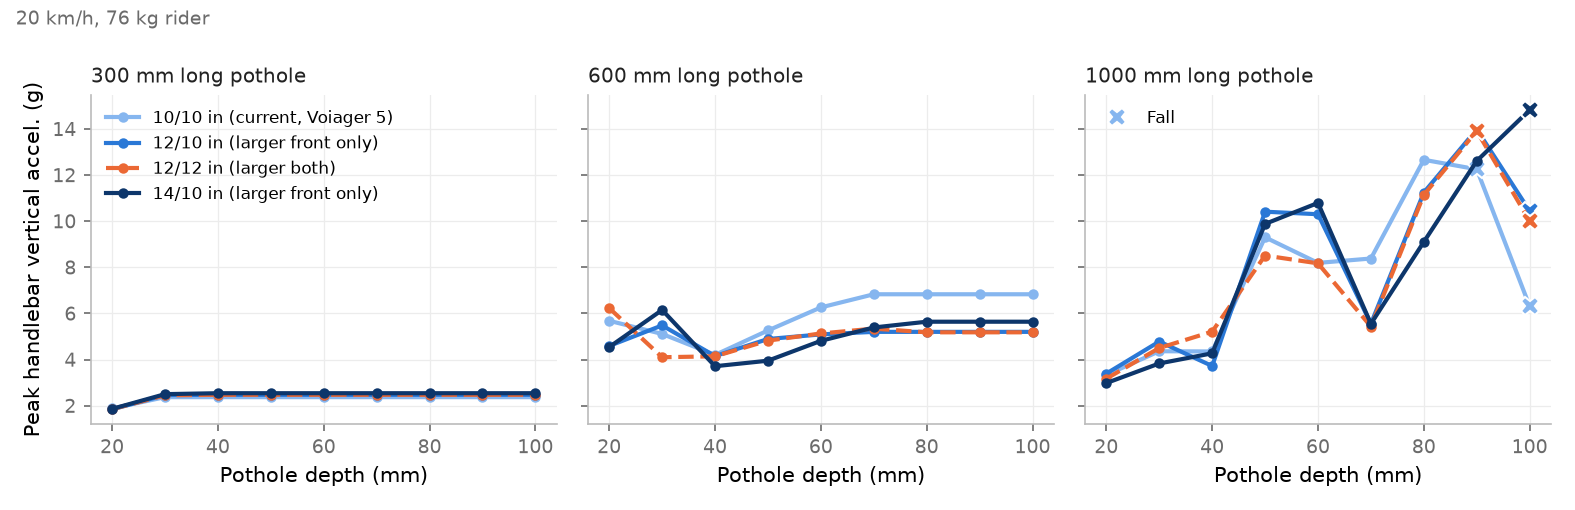
\includegraphics[width=\linewidth]{sim/sweep_handlebar_fork.png}
\caption{Main sweep, with front suspension (main model): simulated handlebar peak acceleration. Absolute values are consistent with the rides only for short potholes with the fork (Figure~\ref{fig:consistency}). Planar model with assumed parameters (Table~\ref{tab:4}); relative comparison of wheel configurations only, not real-world thresholds.}\label{fig:Egfork}
\end{figure}

\begin{figure}[htbp]
\centering
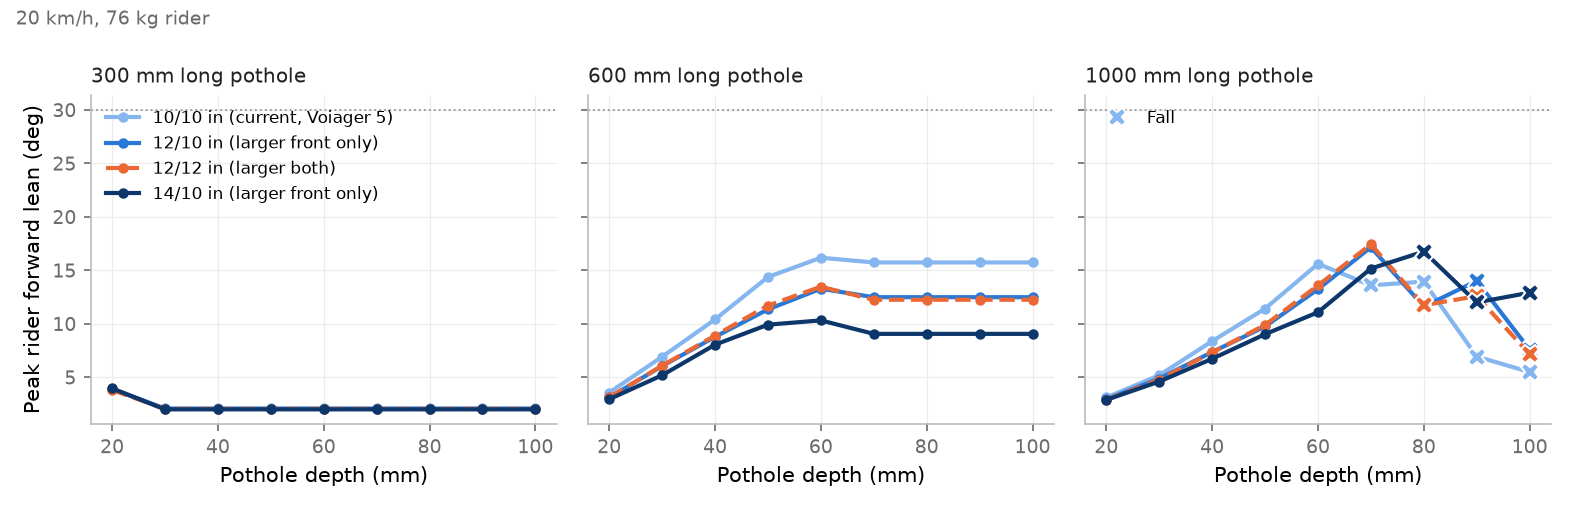
\includegraphics[width=\linewidth]{sim/sweep_lean_nofork.png}
\caption{Main sweep, without suspension: peak forward lean of the rider by pothole depth and length at 20 km/h; X marks a fall. Planar model with assumed parameters (Table~\ref{tab:4}); relative comparison of wheel configurations only, not real-world thresholds.}\label{fig:Eleannofork}
\end{figure}

\begin{figure}[htbp]
\centering
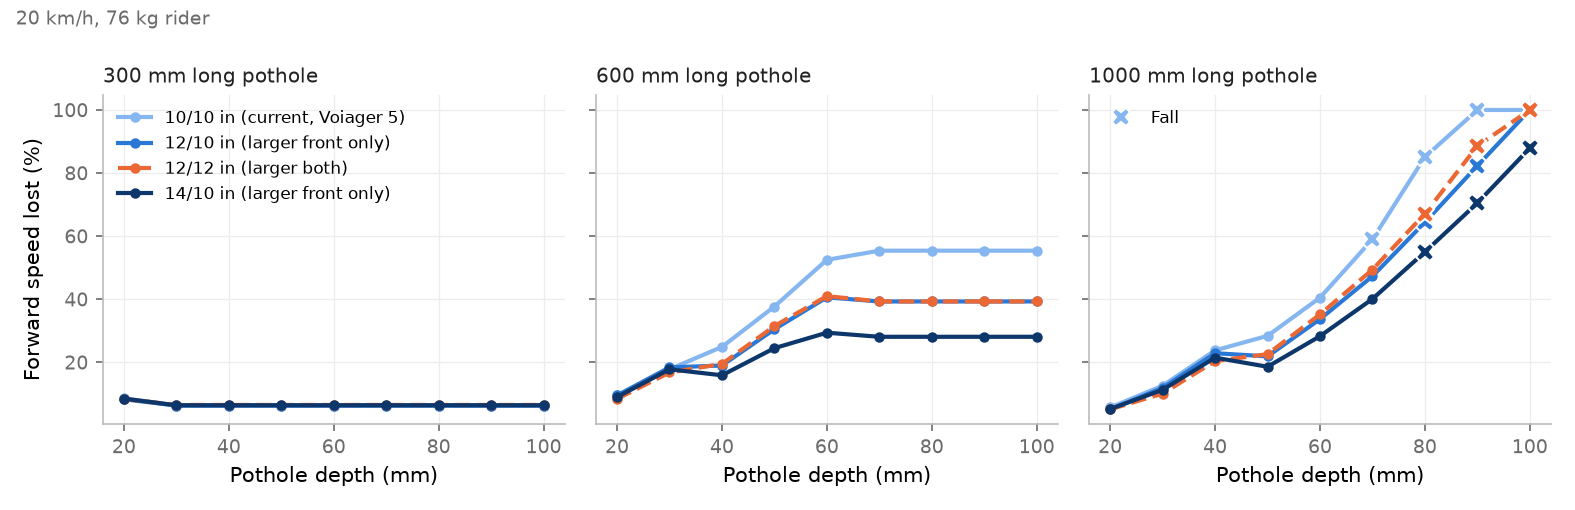
\includegraphics[width=\linewidth]{sim/sweep_speedloss_nofork.png}
\caption{Main sweep, without suspension: forward speed lost crossing the pothole. Planar model with assumed parameters (Table~\ref{tab:4}); relative comparison of wheel configurations only, not real-world thresholds.}\label{fig:Espeednofork}
\end{figure}

\begin{figure}[htbp]
\centering
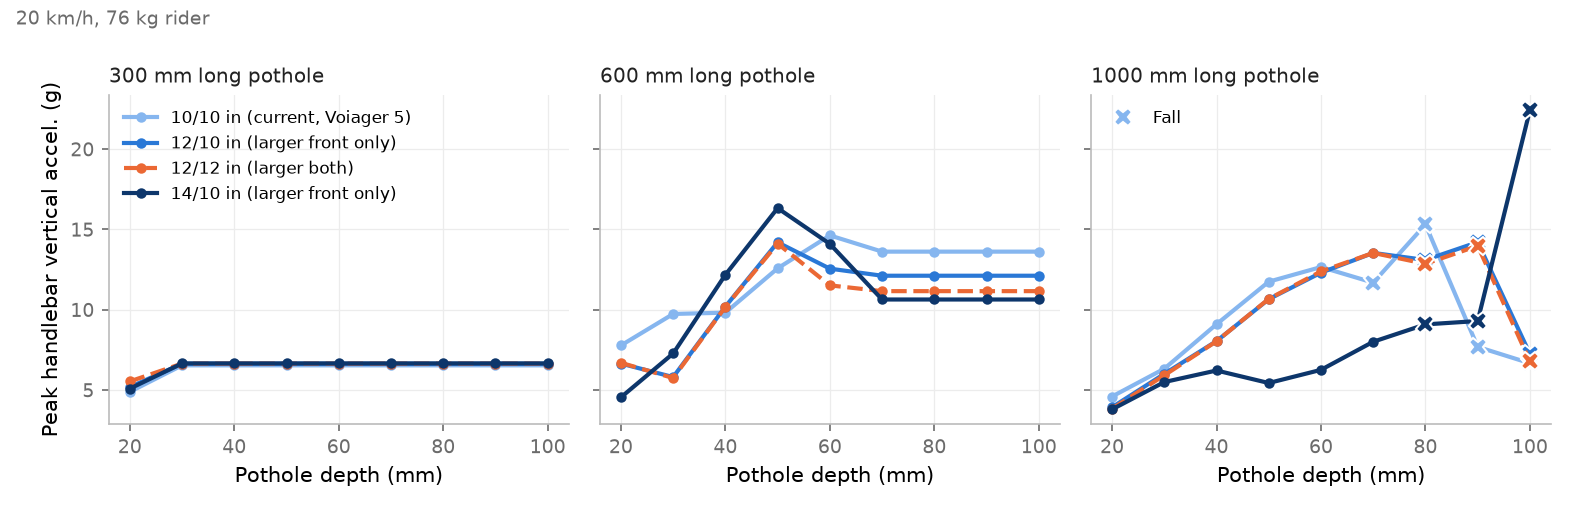
\includegraphics[width=\linewidth]{sim/sweep_handlebar_nofork.png}
\caption{Main sweep, without suspension: simulated handlebar peak acceleration. Absolute values are consistent with the rides only for short potholes with the fork (Figure~\ref{fig:consistency}). Planar model with assumed parameters (Table~\ref{tab:4}); relative comparison of wheel configurations only, not real-world thresholds.}\label{fig:Egnofork}
\end{figure}

\FloatBarrier
\subsection{Front/rear ratio study}

\begin{figure}[htbp]
\centering
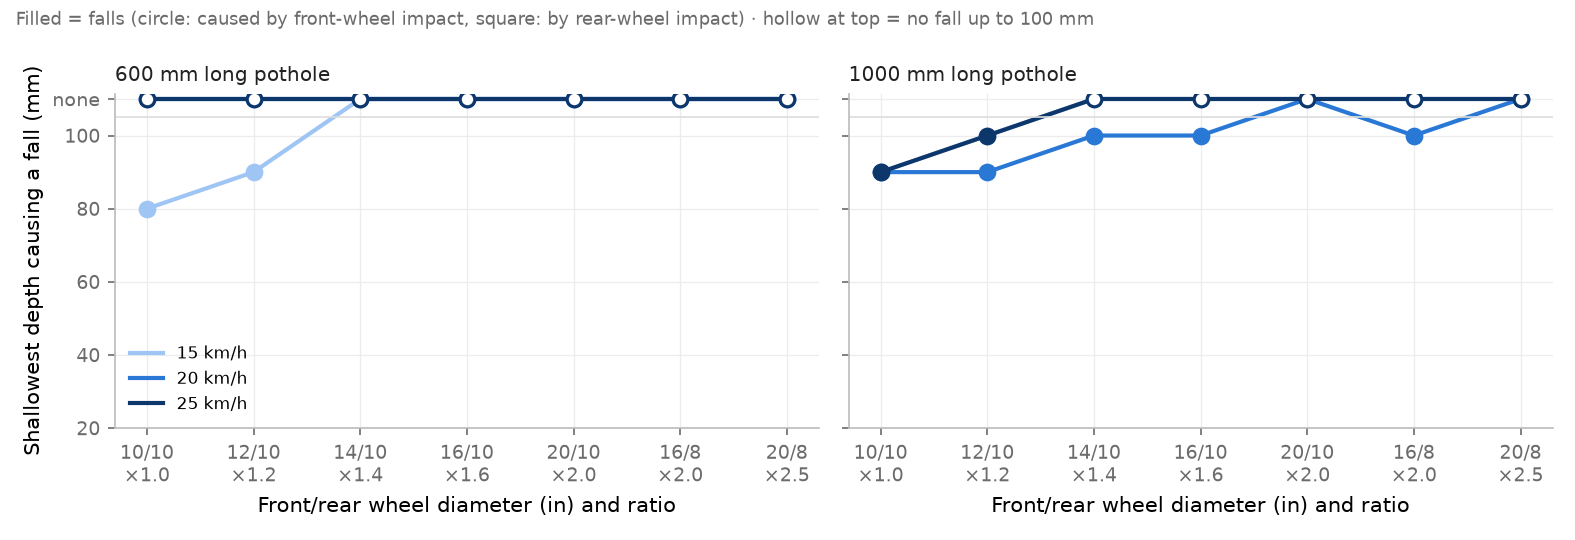
\includegraphics[width=\linewidth]{sim/ratio_first_fall_fork.png}
\caption{Ratio study, with front suspension: shallowest pothole depth (10 mm steps) at which the model fell, by front/rear diameter and speed; ``none'' = no fall up to 100 mm. No ``too large'' front wheel appeared in this planar model, which omits steering, frame geometry and cost. Planar model with assumed parameters (Table~\ref{tab:4}); relative comparison of wheel configurations only, not real-world thresholds.}\label{fig:Eratiofork}
\end{figure}

\begin{figure}[htbp]
\centering
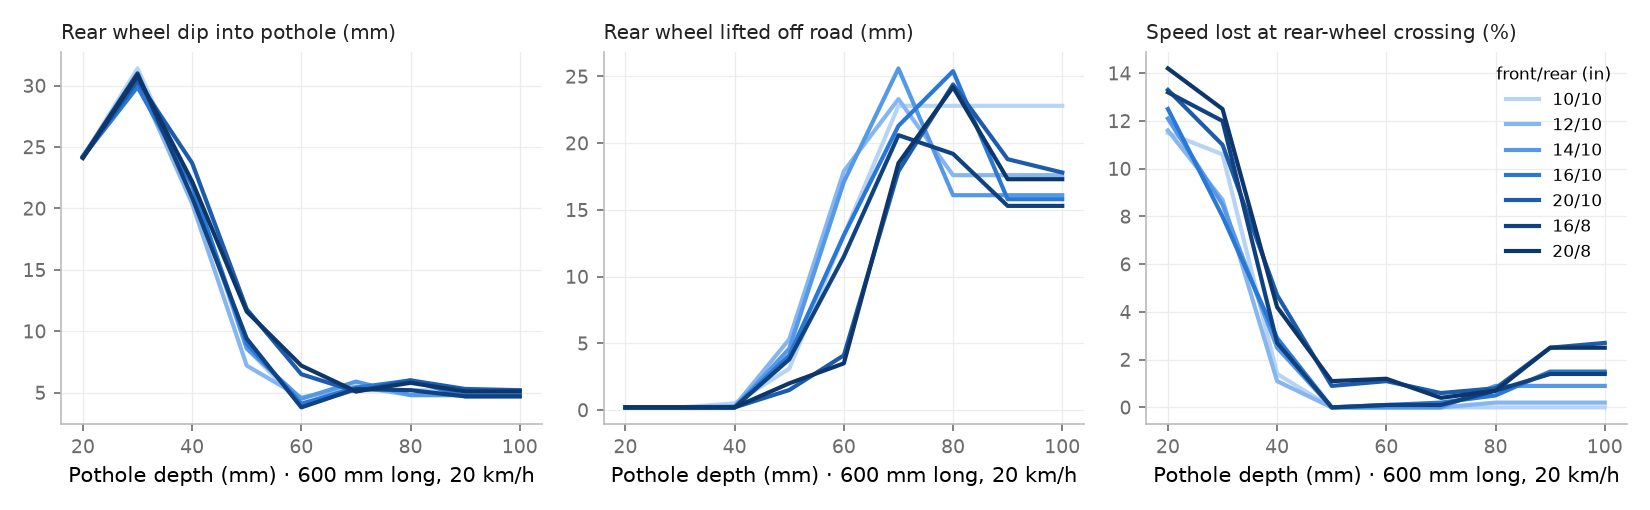
\includegraphics[width=\linewidth]{sim/ratio_rear_wheel_fork.png}
\caption{Ratio study, with front suspension: rear-wheel behaviour on a 600 mm pothole at 20 km/h (dip into the pothole, lift off the road, speed lost at the rear crossing). With the fork the configurations differ little, and the rear wheel is lifted by at most about 25 mm. Planar model with assumed parameters (Table~\ref{tab:4}); relative comparison of wheel configurations only, not real-world thresholds.}\label{fig:Erearfork}
\end{figure}

\begin{figure}[htbp]
\centering
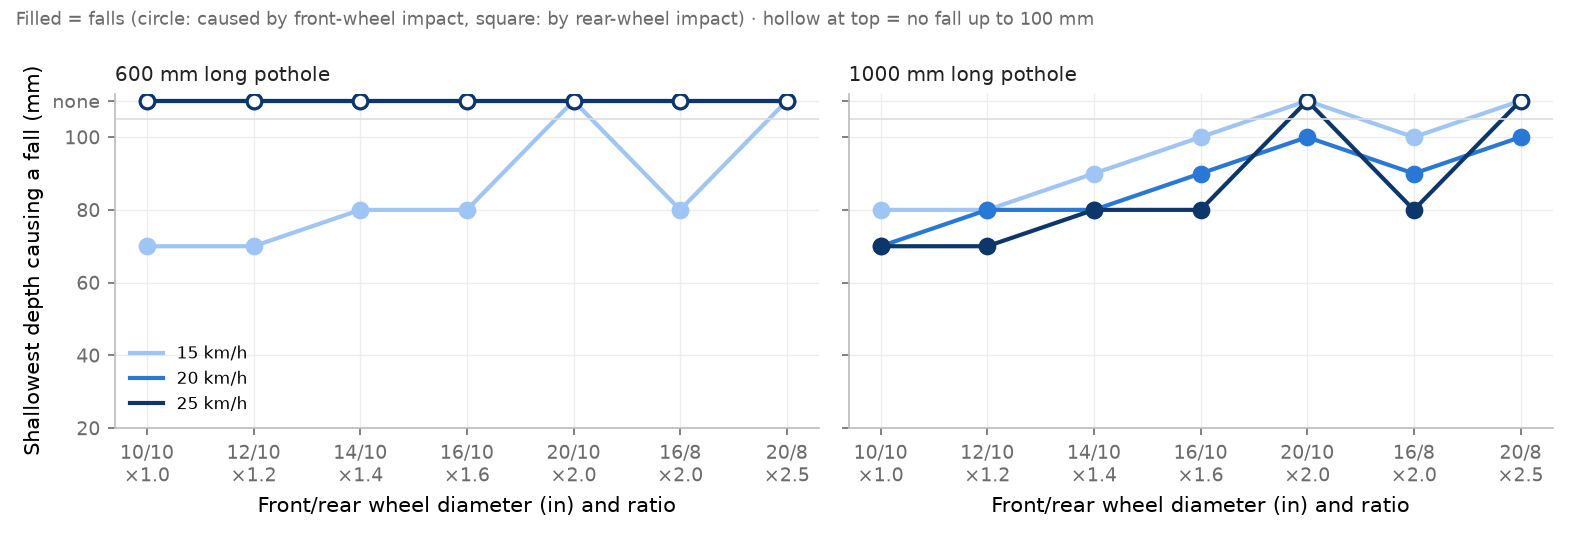
\includegraphics[width=\linewidth]{sim/ratio_first_fall_nofork.png}
\caption{Ratio study, without suspension: shallowest pothole depth (10 mm steps) at which the model fell, by front/rear diameter and speed; ``none'' = no fall up to 100 mm. No ``too large'' front wheel appeared in this planar model, which omits steering, frame geometry and cost. Planar model with assumed parameters (Table~\ref{tab:4}); relative comparison of wheel configurations only, not real-world thresholds.}\label{fig:Erationofork}
\end{figure}

\begin{figure}[htbp]
\centering
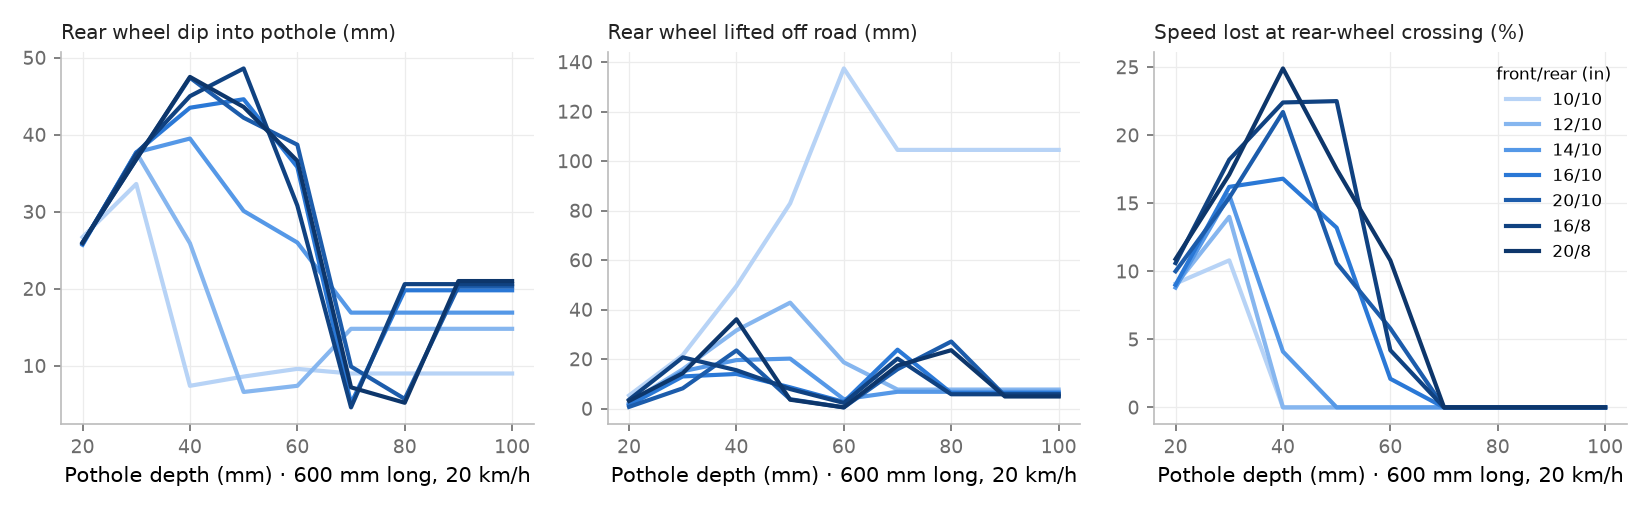
\includegraphics[width=\linewidth]{sim/ratio_rear_wheel_nofork.png}
\caption{Ratio study, without suspension: rear-wheel behaviour on a 600 mm pothole at 20 km/h (dip into the pothole, lift off the road, speed lost at the rear crossing). With small front wheels the rear is lifted clear; with large ones it drops in and gives a second jolt, which caused no falls here. Planar model with assumed parameters (Table~\ref{tab:4}); relative comparison of wheel configurations only, not real-world thresholds.}\label{fig:Erearnofork}
\end{figure}

\FloatBarrier
\subsection{Soft pothole edges}

\begin{figure}[htbp]
\centering
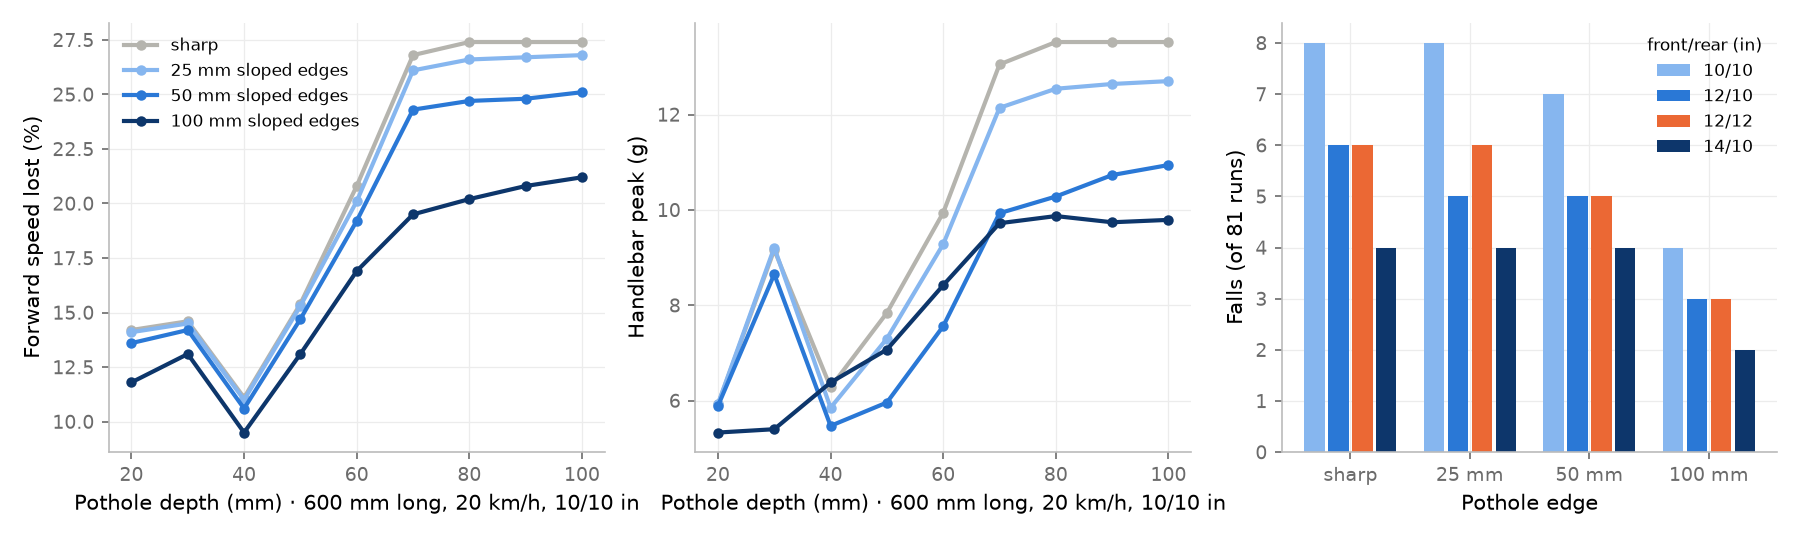
\includegraphics[width=\linewidth]{sim/soft_edges_fork.png}
\caption{Sloped (raised-cosine) pothole edges, with front suspension, profile contact model: speed lost and handlebar peak for 10/10 (600 mm, 20 km/h), and falls of 81 runs per configuration by edge width. The profile contact's absolute accelerations are too high (no tyre enveloping) and are used only for comparison between edge widths. Planar model with assumed parameters (Table~\ref{tab:4}); relative comparison of wheel configurations only, not real-world thresholds.}\label{fig:Eedges}
\end{figure}
\FloatBarrier
\subsection{Summary tables}

The tables below give the fall thresholds without suspension and the sensitivity analysis behind the statements in the model sections. Depths are on a 10 mm grid: ``80'' means a first fall between 70 and 80 mm. -- = no fall up to the deepest case simulated (100 mm). Rows in which no configuration fell are left out. All values come from the planar model with assumed parameters (Table~\ref{tab:4}) and compare configurations; they are not real-world thresholds.

% outputs/scooter_sim/fall_thresholds.csv, sim_results.csv
\begin{table}[htbp]
\centering\small
\caption{Shallowest pothole depth (mm) causing a fall, model without suspension (counterpart of Table~\ref{tab:7}). 11/10 (V5) = the Voi Voiager 5 that was ridden; 10/10 (ref.) = smaller reference wheels.}\label{tab:Enofork}
\begin{tabular}{@{}lrrrrr@{}}
\toprule
Length, speed & 10/10 (ref.) & 11/10 (V5) & 12/10 & 12/12 & 14/10 \\
\midrule
600 mm, 15 km/h & 70 & 70 & 70 & 70 & 80 \\
1000 mm, 15 km/h & 80 & 80 & 80 & 80 & 90 \\
1000 mm, 20 km/h & 70 & 70 & 80 & 80 & 80 \\
1000 mm, 25 km/h & 70 & 70 & 70 & 70 & 80 \\
\textbf{Falls (of 81 runs)} & \textbf{15} & \textbf{15} & \textbf{14} & \textbf{14} & \textbf{11} \\
\bottomrule
\end{tabular}
\end{table}

% outputs/scooter_sim/suspension/sensitivity.csv
\begin{table}[htbp]
\centering\small
\caption{Sensitivity analysis, with front suspension (main model): first fall depth (mm) on a 1000 mm pothole at 20 km/h / forward speed lost on a 60 mm deep, 600 mm pothole at 20 km/h. One parameter changed at a time from the baseline. 11/10 (V5) = the Voi Voiager 5 that was ridden; 10/10 (ref.) = smaller reference wheels.}\label{tab:Esensfork}
\begin{tabular}{@{}p{40mm}rrrrr@{}}
\toprule
Setting & 10/10 (ref.) & 11/10 (V5) & 12/10 & 12/12 & 14/10 \\
\midrule
baseline & 90 / 27.6\% & 90 / 26.8\% & 90 / 25.5\% & 90 / 28.7\% & 100 / 23.2\% \\
stiffer tyre ($\tau$ 0.015 s) & 90 / 30.2\% & 90 / 26.8\% & 90 / 25.1\% & 90 / 25.7\% & 90 / 26.3\% \\
softer tyre ($\tau$ 0.035 s) & 80 / 27.4\% & 90 / 26.7\% & 90 / 23.5\% & 90 / 23.7\% & 90 / 20.6\% \\
weaker bracing (1000 N m/rad) & 90 / 27.8\% & 90 / 29.9\% & 90 / 26.4\% & 90 / 24.7\% & 90 / 21.3\% \\
stronger bracing (3000 N m/rad) & 90 / 28.1\% & 90 / 28.3\% & 90 / 25.4\% & 90 / 25.5\% & 100 / 22.2\% \\
softer fork (15 kN/m) & 80 / 26.5\% & 80 / 24.1\% & 90 / 25.8\% & 90 / 24.6\% & 90 / 22.1\% \\
stiffer fork (40 kN/m) & 90 / 32.7\% & 90 / 25.8\% & 90 / 26.1\% & 90 / 26.9\% & 100 / 21.3\% \\
less fork damping (ratio 0.15) & 80 / 24.8\% & 80 / 24.9\% & 80 / 24.0\% & 80 / 25.4\% & 80 / 22.4\% \\
more fork damping (ratio 0.5) & 90 / 31.1\% & 90 / 29.0\% & 90 / 25.5\% & 100 / 25.4\% & 100 / 22.4\% \\
\bottomrule
\end{tabular}
\end{table}

% outputs/scooter_sim/sensitivity.csv
\begin{table}[htbp]
\centering\small
\caption{Sensitivity analysis, without suspension: first fall depth (mm) on a 1000 mm pothole at 20 km/h / forward speed lost on a 60 mm deep, 600 mm pothole at 20 km/h. One parameter changed at a time from the baseline. 11/10 (V5) = the Voi Voiager 5 that was ridden; 10/10 (ref.) = smaller reference wheels.}\label{tab:Esensnofork}
\begin{tabular}{@{}p{40mm}rrrrr@{}}
\toprule
Setting & 10/10 (ref.) & 11/10 (V5) & 12/10 & 12/12 & 14/10 \\
\midrule
baseline & 70 / 52.5\% & 70 / 47.4\% & 80 / 40.6\% & 80 / 41.0\% & 80 / 29.4\% \\
stiffer tyre ($\tau$ 0.015 s) & 60 / 69.9\% & 70 / 60.4\% & 70 / 52.4\% & 70 / 52.9\% & 80 / 36.2\% \\
softer tyre ($\tau$ 0.035 s) & 70 / 42.2\% & 80 / 38.1\% & 80 / 33.7\% & 80 / 33.4\% & 90 / 26.0\% \\
weaker bracing (1000 N m/rad) & 70 / 52.7\% & 80 / 47.9\% & 80 / 41.0\% & 80 / 42.9\% & 90 / 29.9\% \\
stronger bracing (3000 N m/rad) & 70 / 51.5\% & 70 / 45.7\% & 80 / 38.7\% & 80 / 40.0\% & 80 / 26.2\% \\
\bottomrule
\end{tabular}
\end{table}

